\section{Methodology}

\subsection{Problem Formulation}
\label{sec:method_overview}

We formulate long-form video anomaly understanding as an \textbf{Intra-Video Retrieval} problem. Given a long video $V$ with $T$ frames, the final task is to predict a video-level label $y\in\{0,1\}$ and a semantic rationale $r$. Candidate intervals are an intermediate evidence interface rather than calibrated frame-level predictions.
Unlike direct single-pass inference, ATR uses two calls:
\begin{equation}
    \mathcal{C} = \text{Scout}(V, \mathcal{Q}_{detect}), \qquad
% \end{equation}
% \begin{equation}
    (y,r) = \text{Sniper}(V, \mathcal{C}, \mathcal{Q}_{verify})
\end{equation}
where $\mathcal{C}$ is a set of semantically retrieved candidate intervals. Crucially, the second call retains $V$ in full and adds a focused view derived from $\mathcal{C}$ (Figure~\ref{fig:framework}); ATR therefore does not replace the video with a truncated clip.

\subsection{Scout for Semantic Candidate Retrieval}
\label{sec:scout}

The Scout module scans the temporally sampled complete video $V_{global}$ and returns semantically suspicious regions of interest. We treat Scout as a candidate retriever, not as a calibrated frame-level temporal localizer.
\textbf{Input Construction}:
\begin{equation}
  \text{Input}_{\text{scout}} = [V_{\text{global}},\; Q_{\text{detect}}]
  \label{eq:scout_input}
\end{equation}
Both $V_{\text{global}}$ and, later, $V_{\text{clip}}$ are processed by the VLM's default temporal sampling strategy, which allocates frames proportional to source duration under a fixed visual token budget. Because $V_{\text{clip}}$ covers only the candidate interval, its frames are entirely concentrated on the anomalous region, producing the \textbf{Temporal Zoom-in} effect described in Section~\ref{sec:input}: the anomaly-context ratio within the clip is drastically higher than that of the global view.



$Q_{\text{detect}}$ instructs the model to scan the video and return \emph{all} potentially anomalous intervals in structured JSON format:
\begin{small}
\begin{verbatim}
[{"start":"MM:SS","end":"MM:SS",
  "reason":"...","confidence":"high/med/low"}]
\end{verbatim}
\end{small}
\noindent We test three prompt strategies that vary the detection bias injected into Scout.
\textbf{Aggressive} adopts a security-guard persona with an exhaustive list of anomaly categories and instructs the model to report all suspicious segments, including low-confidence ones.
\textbf{Minimal} provides only a concise task description without role-play or category enumeration.
\textbf{Neutral} supplies the same category list as Aggressive but adds contextual filtering rules that require distinguishing normal activities from genuinely suspicious behavior.
The optimal strategy varies by model scale (Section~\ref{sec:prompt_ablation}).

\textbf{Candidate Retention.}
All candidates returned by Scout are retained regardless of confidence.
Overlapping or adjacent intervals within a 2\,s gap are merged:
if $t_{\text{start}}^{j} \leq t_{\text{end}}^{i} + 2$, intervals $i$ and $j$ are fused into a single interval.
When Scout returns an empty list, ATR follows a conservative fallback and returns the independently computed global-only baseline judgment. This path cannot create ATR's gains because it adds no local evidence.

\textbf{Output}: A set of candidate timestamps $\mathcal{C} = \{(t_{\text{start}}^i, t_{\text{end}}^i)\}_{i=1}^N$.

\subsection{Sniper for Focused Anomaly Verification}
\label{sec:sniper}

The Sniper module performs the core reasoning. It receives focused evidence retrieved from the source video and jointly reasons over the global and local views.

\subsubsection{Temporal Context Padding}
\label{sec:ace}

Before clip extraction, we add a fixed amount of surrounding temporal context:
\begin{align}
  t'_{\text{start}} &= \max(0,\; t_{\text{start}} - \Delta_{\text{pre}}) \label{eq:ace_start}\\
  t'_{\text{end}}   &= t_{\text{end}} + \Delta_{\text{post}} \label{eq:ace_end}
\end{align}
We retain the originally frozen setting $\Delta_{\text{pre}} = 10$\,s and $\Delta_{\text{post}} = 2$\,s for reproducibility. Equal-budget controls compare $0/0$, $6/6$, $10/2$, and $2/10$ padding on the same Scout candidates (Table~\ref{tab:ace_ablation}). The two directional variants obtain identical balanced accuracy for both evaluated model scales, showing that ATR does not depend on a finely tuned asymmetric boundary. Padding is therefore an implementation detail rather than a separate mechanism.
The clip is extracted from the source video via \texttt{ffmpeg} stream-copy (no re-encoding), preserving the original codec and frame timing.

\subsubsection{Hierarchical Visual Input Construction}
\label{sec:input}

ATR constructs a heterogeneous input sequence that encourages the model to attend to both the forest and the trees:
\begin{equation}
  \text{Input}_{\text{sniper}} = [V_{\text{global}},\; \text{Sep}_1,\; V_{\text{clip}},\; \text{Sep}_2,\; Q_{\text{verify}}]
  \label{eq:sniper_input}
\end{equation}

Here $V_{\text{global}}$ is the same complete original video used by Scout, while $V_{\text{clip}}$ is cut from that video. Both are supplied together in the Sniper call. The local clip therefore adds a second evidence view without removing any global temporal context.

\textbf{Mechanism 1: Temporal Zoom-in}.
By presenting $V_{clip}$ alongside $V_{global}$, ATR achieves a \textbf{Temporal Zoom-in} effect. 
% Even without increasing the physical frame rate, replacing a long video with a short focused clip drastically elevates the \textbf{Anomaly Context Ratio} (from $\sim$1.6\% to $\sim$13.3\% in our experiments, see Figure~\ref{fig:temporal_zoom}). 
In the illustrative example shown in Figure~\ref{fig:temporal_zoom}, replacing a long video with a short focused clip increases the anomaly-context ratio from $\sim$1.6\% to $\sim$13.3\% (computed as anomaly duration over total source duration).
This redistribution of evidence density makes candidate frames easier to revisit under a limited visual-token budget.

\textbf{Connection to Prompt Repetition}.
For a causal language model, tokens in a later repeated copy can attend to the earlier copy, reducing order sensitivity and creating a re-reading path~\cite{leviathan2025prompt}. ATR transfers this intuition to visual evidence without repeating the entire video: Scout-selected content is presented again as a short second view, while the complete video remains available. The mechanism is a design motivation rather than a theoretical guarantee for VLM attention; Section~\ref{sec:module_ablation} therefore tests it empirically using Clip-Only and relevance-controlled inputs.

\textbf{Source-role instructions}.
The separators carry explicit role assignments:
\begin{small}
\begin{itemize}
  \item $\text{Sep}_1$: \texttt{"SOURCE 1: Global Context (Low FPS). Use this ONLY to understand the setting (e.g., store, street)."}
  \item $\text{Sep}_2$: \texttt{"SOURCE 2: Local Detail (High FPS, Focused Clip). This clip contains the CRITICAL MOMENT."}
\end{itemize}
\end{small}
\noindent These separators identify the intended role of each visual source: Source~1 supplies scene context and Source~2 supplies concentrated candidate evidence. Full prompt texts for all three strategies are provided in Appendix~A. The ``High/Low FPS'' wording is an instruction cue rather than a claim that every backend uses a literal frame-rate differential.




\begin{figure}[t]
  \centering
  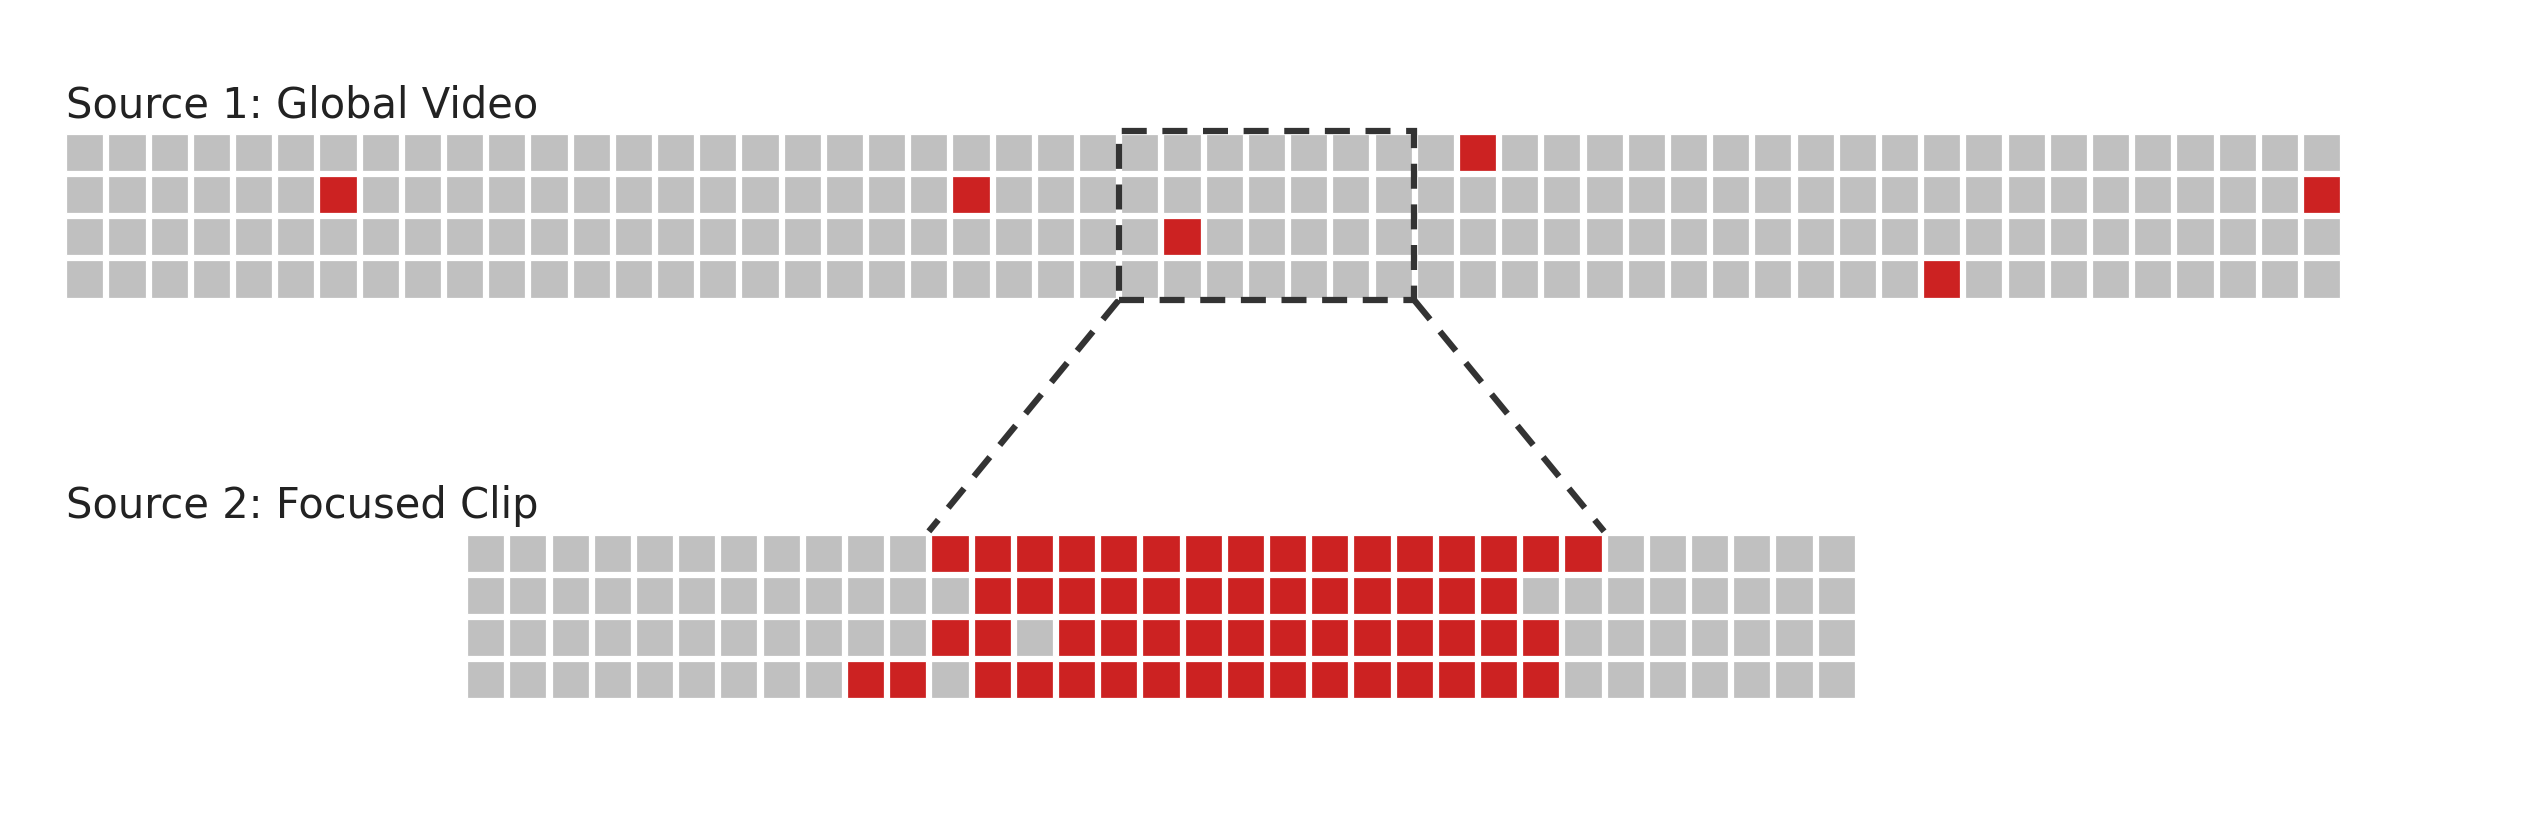
\includegraphics[width=\columnwidth]{figures/fig_temporal_zoomin.png}
  \caption{Temporal Zoom-in effect. Source~1 is the complete video; the small squares denote temporally sampled frames/visual tokens distributed over its full timeline, not object proposals. Source~2 is a clip cut from the Scout candidate window and sampled separately. In this example, the annotated anomaly occupies $\sim$1.6\% of Source~1 but $\sim$13.3\% of Source~2. Both sources are jointly provided to Sniper.}
  \label{fig:temporal_zoom}
\end{figure}

\subsection{Interaction-Aware Reasoning Prompt}
\label{sec:prompt}

To encourage explicit verification, we use a three-step structured reasoning prompt~\cite{wang2022self,yao2023tree}:


(1) \textbf{Observation}: Describe micro-actions in Source~2 (hand movements, body language).
(2) \textbf{Context Analysis}: Use Source~1 to identify environment and behavioral norms.
(3) \textbf{Classification}: Match against known anomaly patterns, explicitly \textbf{ruling out alternative benign explanations} (e.g., ``play fighting'' vs. ``assault'').

Compared to full video repetition ($V \oplus V$), ATR only repeats a short critical segment
($V \oplus \delta$); token overhead and efficiency comparisons are detailed in
Section~\ref{sec:discussion}.
